\clearpage
\subsection{Making the Hello World Program} % (fold)
\label{sub:compiling_code}

\lref{lst:hello-world-c} and \lref{lst:hello-world-pas} show the source code for the Hello World program. To make this into a program you need to:

\begin{enumerate}
  \item Write the code into a text file.
  \item Save the text file to disk.
  \item Compile it.
\end{enumerate}

Step 1 and 2 can be accomplished with any text editor, but the best ones to use highlight your code. Each programming language has rules that determine how its code must be formatted. This is known as the language's \textbf{syntax}. You can get text editors that understand these rules, and highlight your code as you type. This is called \textbf{syntax highlighting}. This highlighting can help you identify any little mistakes you make. \fref{fig:linux-editors} shows the Hello World code in gedit in Linux. \fref{fig:mac-editors} shows the code in TextMate on Mac OS. \fref{fig:windows-editors} shows the code in Notepad++ in Windows.

\begin{figure}[h]
   \centering
   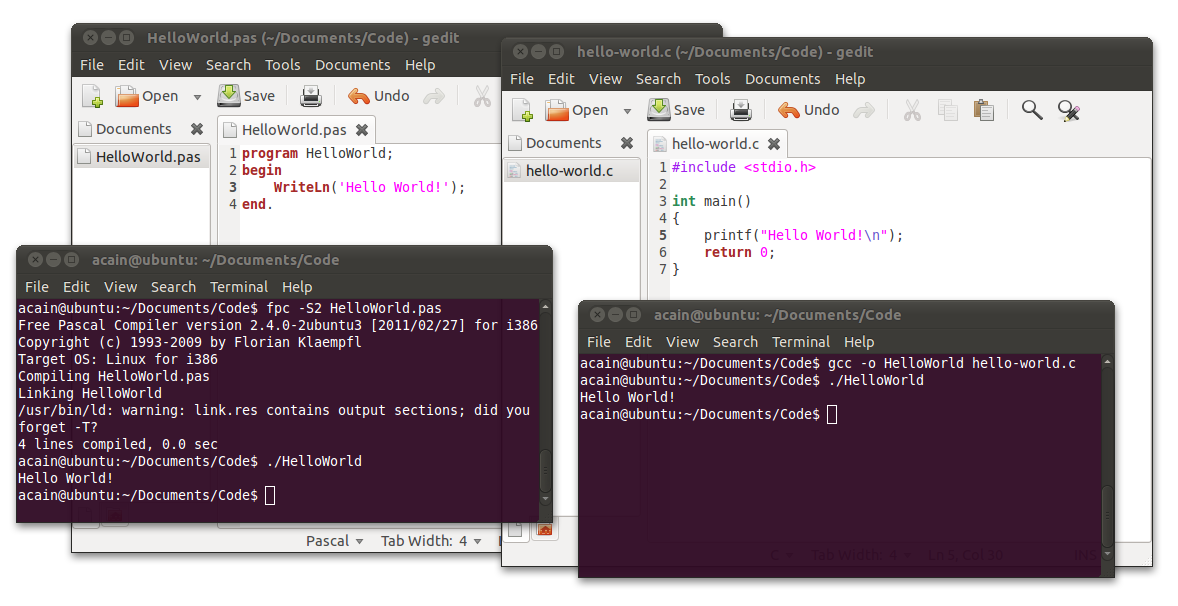
\includegraphics[width=\textwidth]{./topics/programs-and-compilers/images/LinuxEditors} 
   \caption{Editing and Compiling C and Pascal code in Linux}
   \label{fig:linux-editors}
\end{figure}

\begin{figure}[h]
   \centering
   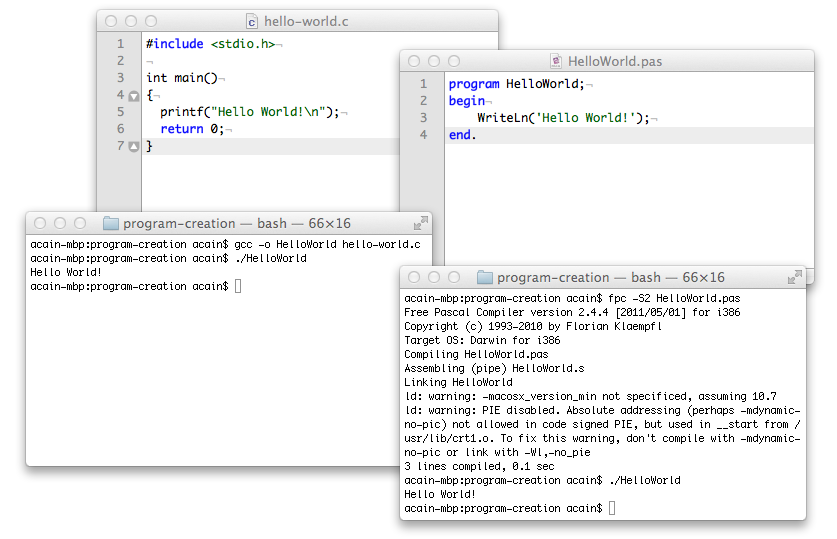
\includegraphics[width=\textwidth]{./topics/programs-and-compilers/images/MacEditors} 
   \caption{Editing and Compiling C and Pascal code in Mac OS}
   \label{fig:mac-editors}
\end{figure}

\begin{figure}[h]
   \centering
   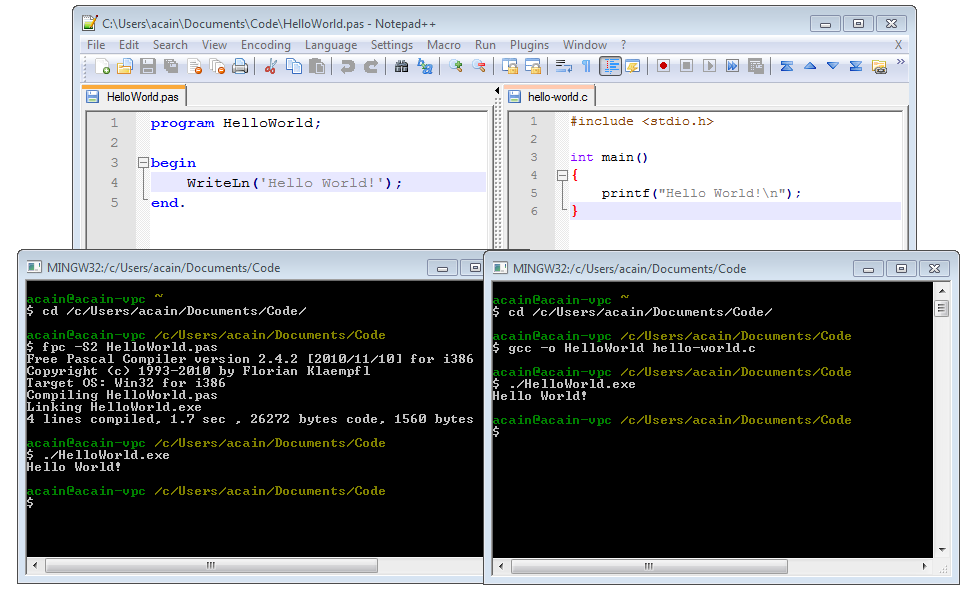
\includegraphics[width=\textwidth]{./topics/programs-and-compilers/images/WindowsEditors} 
   \caption{Editing and Compiling C and Pascal code in Windows}
   \label{fig:windows-editors}
\end{figure}


\mynote{
\begin{itemize}
  \item Syntax highlighting editors include:
  \begin{itemize}
    \item \textbf{gedit} on Linux.
    \item \textbf{TextMate} or \textbf{TextWrangler} on MacOS.
    \item \textbf{Notepad++} or \textbf{Crimson Editor} on Windows.
  \end{itemize}
  \item Take care when you type the code in, even one character out of place may mean the compiler fails to compile your code.
\end{itemize}
}

\clearpage
\subsubsection{Running the Compiler} % (fold)
\label{ssub:running_the_compiler}

When you run the compiler you will pass to it two kinds of information: options, and the file or files you want converted to machine code. The compiler will read the files you pass it and use the language's syntax to determine the tasks you want performed. Once it has built up a model of the program it will the write machine code instructions into a program file. When the compiler finishes you can then run the program file and see the computer perform the tasks coded in the source code.

\csection{
\bashcode{lst:compile-hello-world-c}{Compiling C code.}{code/c/program-creation/compile-hello-world.sh}

There are many different C compilers. The one we will use is the \textbf{gcc} compiler, the \textbf{GNU C Compiler} as shown in Listing \ref{lst:compile-hello-world-c}. When you call the compiler you can use the \emph{-o name} option to tell it the name of the program file to create. In our example this will compile the code in \emph{hello-world.c} and save the machine code into a program called \emph{HelloWorld}.}

\passection{
\bashcode{lst:compile-hello-world-pas}{Compiling Pascal code.}{code/pascal/program-creation/compile-hello-world.sh}

Listing \ref{lst:compile-hello-world-pas} shows the instructions to run the \textbf{fpc} compiler. FPC is the \textbf{Free Pascal Compiler}, which can compile a number of different versions of the Pascal language. The \emph{-S2} option is used to tell FPC to compile using the latest `Free Pascal' version of the language. In our example this will compile the code in \emph{HelloWorld.pas} and save the machine code into a program called \emph{HelloWorld}, which it gets from the name of the Pascal file.}

If the source code you try to compile does not follow all of the rules of the language then the compiler will end with an error message. These errors, called \textbf{syntax errors}, could be as small as missing a semicolon (;), or misspelling a name. When the compiler encounters these issues it does not create the executable program, but instead returns a list showing where it got to before it found an error. You can use these error messages to fix the mistakes, and then run the compiler again to generate your program.


% subsubsection running_the_compiler (end)
% section the_compiler (end)
